%%
%% getstart.tex -- Flight Gear documentation: Installation and Getting Started
%% Chapter file
%%
%% Copyright (C) 2002 Michael Basler (pmb@epost.de)
%%                  & Bernhard Buckel (buckel@wmad95.mathematik.uni-wuerzburg.de)
%%
%% This program is free software; you can redistribute it and/or
%% modify it under the terms of the GNU General Public License as
%% published by the Free Software Foundation; either version 2 of the
%% License, or (at your option) any later version.
%%
%% This program is distributed in the hope that it will be useful, but
%% WITHOUT ANY WARRANTY; without even the implied warranty of
%% MERCHANTABILITY or FITNESS FOR A PARTICULAR PURPOSE.  See the GNU
%% General Public License for more details.
%%
%% You should have received a copy of the GNU General Public License
%% along with this program; if not, write to the Free Software
%% Foundation, Inc., 675 Mass Ave, Cambridge, MA 02139, USA.
%%
%% $Id: takeof.tex,v 0.5 2002/15/02 michael
%% (Log is kept at end of this file)

%%%%%%%%%%%%%%%%%%%%%%%%%%%%%%%%%%%%%%%%%%%%%%%%%%%%%%%%%%%%%%%%%%%%%%%%%%%%%%%%%%%%%%%%%%%%%%%%%
\chapter{Takeoff: How to start the program\label{takeoff}}
%%%%%%%%%%%%%%%%%%%%%%%%%%%%%%%%%%%%%%%%%%%%%%%%%%%%%%%%%%%%%%%%%%%%%%%%%%%%%%%%%%%%%%%%%%%%%%%%%
\markboth{\thechapter.\hspace*{1mm}
TAKEOFF}{\thesection\hspace*{1mm} Command line parameters}
%%%%%%%%%%%%%%%%%%%%%%%%%%%%%%%%%%%%%%%%%%%%%%%%%%%%%%%%%%%%%%%%%%%%%%%%%%%%%%%%%%%%%%%%%%%%%%%%%
\section{Launching the simulator under Unix/Linux}\index{Launching Flightgear!Linux}\index{Starting Flightgear!Linux}
%%%%%%%%%%%%%%%%%%%%%%%%%%%%%%%%%%%%%%%%%%%%%%%%%%%%%%%%%%%%%%%%%%%%%%%%%%%%%%%%%%%%%%%%%%%%%%%%%
Under Linux (or any other flavor of Unix), \FlightGear{} will be invoked by
 \medskip

  \texttt{runfgfs -$ $-option1 -$ $-option2\dots},
 \medskip

\noindent
 where the options will be described in Section \ref{options} below.
 
If something strange happens while using this shell script, if you want to do some
debugging (i.e. using ''strace'') or if you just feel nice to be ''keen'', then you can
start \FlightGear{} directly by executing the ''fgfs'' binary. In this case you should at
least add one variable to your environment,\index{environment variables} which is needed
to locate the (mostly) shared library built from the sources of the \SimGear{}
package. Please add the respective directory to your \verb/LD_LIBRARY_PATH/. You can do
so with the following on Bourne shell (compatibles):

\begin{verbatim}
LD_LIBRARY_PATH=/usr/local/FlightGear/lib:$LD_LIBRARY_PATH
export LD_LIBRARY_PATH/
\end{verbatim}

\noindent
 or on C shell (compatibles):
 
\begin{verbatim}
setenv LD_LIBRARY_PATH
/usr/local/FlightGear/lib:$LD_LIBRARY_PATH
\end{verbatim}

 \noindent
Besides this (used by the dynamic linker) ''fgfs'' knows about the following environment variable:
\noindent

\verb/FG_ROOT/: root directory for the FlightGear base package,

\noindent
 which corresponds to the \texttt{-$ $-fg-root={\it path}} option as described in Sec. \ref{generaloptions}

%%%%%%%%%%%%%%%%%%%%%%%%%%%%%%%%%%%%%%%%%%%%%%%%%%%%%%%%%%%%%%%%%%%%%%%%%%%%%%%%%%%%%%%%%%%%%%%%%
\section{Launching the simulator under Windows}\index{Launching Flighgear!Windows}\index{Starting Flightgear!Windows}
%%%%%%%%%%%%%%%%%%%%%%%%%%%%%%%%%%%%%%%%%%%%%%%%%%%%%%%%%%%%%%%%%%%%%%%%%%%%%%%%%%%%%%%%%%%%%%%%%
For launching \FlightGear{} from Windows explorer, change to the directory \texttt{/FlightGear} and double-click the file \texttt{runfgfs.bat}.
 \medskip

 \centerline{\fbox{
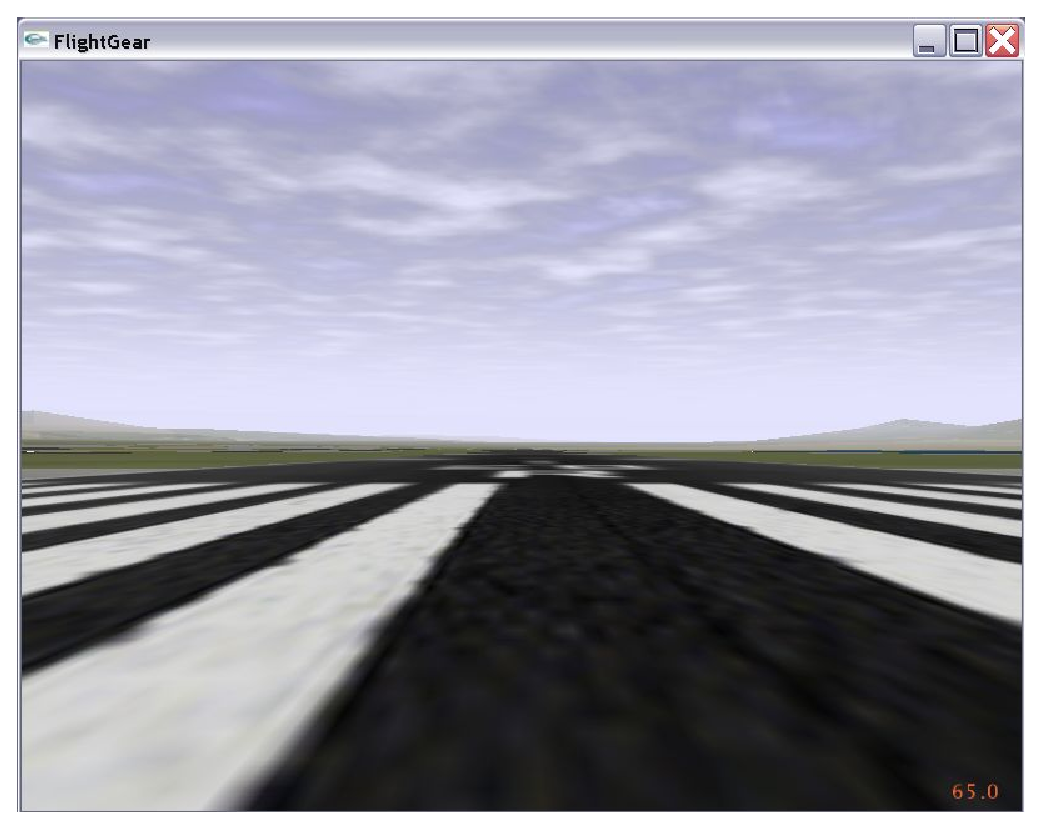
\includegraphics[clip,width=12.5cm]{ksfo}
}}
\smallskip

 \noindent
Fig.\,3: \textit{Ready for takeoff. Waiting at the default startup position at San
Francisco Itl., KSFO.}
\medskip

Alternatively, if for one or the other reason the batch file above does not work or is missing,
you can open a command shell, change to the directory where your binary resides
(typically something like \texttt{c:/FlightGear/bin} where you might have to substitute
\texttt{c:} in favor of your \FlightGear{} directory), set the \Index{environment
variable} via (note the backslashes!)
 \medskip

\texttt{SET FG\_ROOT=c:$\backslash$FlightGear$\backslash$}
 \medskip

\noindent
 and invoke \FlightGear{} (within the same MS-DOS shell, as environment
 settings are only valid locally within the same shell) via
  \medskip

\texttt{fgfs -$ $-option1 -$ $-option2\dots}.
 \medskip

Of course,  you can create your own \texttt{runfgfs.bat} with Windows \texttt{Editor} using the
two lines above.

For getting maximum performance it is recommended to minimize (iconize) the text output
window while running \FlightGear{}$\!$.

%%%%%%%%%%%%%%%%%%%%%%%%%%%%%%%%%%%%%%%%%%%%%%%%%%%%%%%%%%%%%%%%%%%%%%%%%%%%%%%%%%%%%%%%%%%%%%%%%
\section{Launching the simulator under Mac OS X}\index{Launching Flighgear!Mac OS X}\index{Starting Flightgear!Mac OS X}
%%%%%%%%%%%%%%%%%%%%%%%%%%%%%%%%%%%%%%%%%%%%%%%%%%%%%%%%%%%%%%%%%%%%%%%%%%%%%%%%%%%%%%%%%%%%%%%%%
Say, you downloaded the base package and binary to your home directory. Then you can open \texttt{Terminal.app} and execute the following sequence:
\medskip

\noindent
\texttt{setenv FG\_ROOT ~/fgfs-base-X.X.X ./fgfs-X.X.X.-date}\\
\texttt{-$ $-option1 -$ $- option 2} (one line)
\medskip

\noindent
or
\medskip

\noindent
\texttt{./fgfs-X.X.X-version-date}
 \texttt{-$ $-fg-root=\~/fgfs-base-X.X.X}\\
 \texttt{-$ $-option1 -$ $-option2}. (one line)

%%%%%%%%%%%%%%%%%%%%%%%%%%%%%%%%%%%%%%%%%%%%%%%%%%%%%%%%%%%%%%%%%%%%%%%%%%%%%%%%%%%%%%%%%%%%%%%%%
\section{Command line parameters\label{options}}\index{command line options}
%%%%%%%%%%%%%%%%%%%%%%%%%%%%%%%%%%%%%%%%%%%%%%%%%%%%%%%%%%%%%%%%%%%%%%%%%%%%%%%%%%%%%%%%%%%%%%%%%
Following is a list and short description of the numerous \Index{command line options}
available for \FlightGear{}$\!$. If you are running \FlightGear{} under \Index{Windows} you can include these into
\texttt{runfgfs.bat}.

However, in case of options you want to re-use continually it is recommended to include them into a file called
\texttt{.fgfsrc}\index{.fgfsrc} under Unix systems and
\texttt{system.fgfsrc},\index{system.fgfsrc} resp. under Windows. This file has to be in
the top \FlightGear{} directory (for instance /usr/local/Flightgear). As it depends on your
\Index{preferences}, it is not delivered with \FlightGear{}$\!$, but can be created with
any text editor (notepad, emacs, vi, if you like). 

%%%%%%%%%%%%%%%%%%%%%%%%%%%%%%%%%%%%%%%%%%%%%%%%%%%%%%%%%%%%%%%%%%%%%%%%%%%%%%%%%%%%%%%%%%%%%%%%%
\subsection{General Options}\index{options!general}\label{generaloptions}
%%%%%%%%%%%%%%%%%%%%%%%%%%%%%%%%%%%%%%%%%%%%%%%%%%%%%%%%%%%%%%%%%%%%%%%%%%%%%%%%%%%%%%%%%%%%%%%%%
\begin{itemize}
\item{\texttt{-$ $-help}, \texttt{-h}}: Shows the Gives a small help text, kind of a short version of this Section.
\item{\texttt{-$ $-fg-root={\it path}}}: Tells \FlightGear{} where to look for its data
  files if you didn't compile it with the \Index{default settings}.
\item{\texttt{-$ $-fg-scenery={\it path}}}: Allows specification of a path to the scenery
directorypath \index{scenery directory!path}, in case scenery is not at the default
position under\\
 \texttt{/Flightgear/Scenery}; this might be especially useful in case you
have scenery on a CD-ROM.
\item{\texttt{-$ $-disable-game-mode}}: Disables \Index{full screen display}.

\item{\texttt{-$ $-enable-game-mode}}: Enables full screen display.

\item{\texttt{-$ $-disable-splash-screen}}: Turns off the rotating 3DFX logo
 when the accelerator board gets initialized (3DFX only).
\item{\texttt{-$ $-enable-splash-screen}}: If you like advertising, set this!
\item{\texttt{-$ $-disable-intro-music}}: No audio sample is being played when
  \FlightGear{} starts up. Suggested in case of trouble with playing the intro.
\item{\texttt{-$ $-enable-intro-music}}: If your machine is powerful enough, enjoy
  this setting.
\item{\texttt{-$ $-disable-mouse-pointer}}: Disables \Index{mouse interface}.
\item{\texttt{-$ $-enable-mouse-pointer}}: Enables \Index{mouse interface}. Useful in
full screen mode for old Voodoo/VoodooII based cards.
\item{\texttt{-$ $-disable-freeze}}: This will put you into \FlightGear{} with the
  engine running, ready for Take-Off.
\item{\texttt{-$ $-enable-freeze}}: Starts \FlightGear{} in \Index{frozen state}.
\item{\texttt{-$ $-disable-fuel-freeze}}: Fuel is consumed normally.
\item{\texttt{-$ $-enable-fuel-freeze}}: Fuel tank quantity is forced to remain constant.
\item{\texttt{-$ $-disable-tod-freeze}}: Time of day advances normally.
\item{\texttt{-$ $-enable-tod-freeze}}: Do not advance time of day.
\item{\texttt{-$ $-control-mode}}: Specify your \Index{control device} (\Index{joystick},
 keyboard, mouse) Defaults to \Index{joystick} (\Index{yoke}).
\item{\texttt{-$ $-disable-auto-coordination}}: Switches \Index{auto coordination} between
aileron/rudder off (default).
\item{\texttt{-$ $-enable-auto-coordination}}: Switches auto coordination between
aileron/rudder on (recommended without pedals).
\item{\texttt{-$ $-browser-app=/path/to/app}}:  specify location of your web browser. Example:
\texttt{-$ $-browser-app=}\\  \texttt{''C:$\backslash$Programme$\backslash$Internet~Explorer$\backslash$iexplore.exe''} (Note the '' '' because of the broken word Internet Explorer!).
\item{\texttt{-$ $-prop:name=value:}}  set property \texttt{name} to \texttt{value}\\Example:
\texttt{-$ $-prop:/engines/engine0/running=true} for starting with running engines. Another example:\\
\texttt{-$ $-aircraft=c172}\\
\texttt{-$ $-prop:/consumables/fuels/tank[0]/level-gal=10}\\
\texttt{-$ $-prop:/consumables/fuels/tank[1]/level-gal=10}\\
filles the Cessna for a short flight.
\item{\texttt{-$ $-config=path:}}  Load additional properties from the given path. Example: \texttt{runfgfs -$ $-config=./Aircraft/X15-set.xml}
\item{\texttt{-$ $-units-feed}}: Use feet for distances.
\item{\texttt{-$ $-units-meters}}: Use meters for distances.
\end{itemize}
%%%%%%%%%%%%%%%%%%%%%%%%%%%%%%%%%%%%%%%%%%%%%%%%%%%%%%%%%%%%%%%%%%%%%%%%%%%%%%%%%%%%%%%%%%%%%%%%%
\subsection{Features}\index{options!features}
%%%%%%%%%%%%%%%%%%%%%%%%%%%%%%%%%%%%%%%%%%%%%%%%%%%%%%%%%%%%%%%%%%%%%%%%%%%%%%%%%%%%%%%%%%%%%%%%%
\begin{itemize}
\item{\texttt{-$ $-disable-hud}}: Switches off the \Index{HUD} (\textbf{H}ead \textbf{U}p
  \textbf{D}isplay).
\item{\texttt{-$ $-enable-hud}}: Turns the  \Index{HUD} on.
\item{\texttt{-$ $-enable-anti-aliased-hud}}: Turns on \Index{anti-aliaseded HUD lines} for better quality,
if hardware supports this.
\item{\texttt{-$ $-disable-anti-aliased-hud}}: Turns off anti-aliaseded HUD lines.
\item{\texttt{-$ $-enable-panel}}: Turns the \Index{instrument panel} on (default).
\item{\texttt{-$ $-disable-panel}}: Turns the \Index{instrument panel} off.
\item{\texttt{-$ $-disable-sound}}: Self explaining.
\item{\texttt{-$ $-enable-sound}}: See above.
\end{itemize}
%%%%%%%%%%%%%%%%%%%%%%%%%%%%%%%%%%%%%%%%%%%%%%%%%%%%%%%%%%%%%%%%%%%%%%%%%%%%%%%%%%%%%%%%%%%%%%%%%
\subsection{Flight model\index{flight dynamics model}}\index{options!flight model}
%%%%%%%%%%%%%%%%%%%%%%%%%%%%%%%%%%%%%%%%%%%%%%%%%%%%%%%%%%%%%%%%%%%%%%%%%%%%%%%%%%%%%%%%%%%%%%%%%
\begin{itemize}
\item{\texttt{-$ $-aircraft={\it name of aircraft definition file}}} Example: \texttt{-$ $-aircraft=c310}. For possible choices check the directory \texttt{/FlightGear/Aircraft}. Do not include the extension \texttt{''-set.xml''} into the aircraft name but use the remaining beginning of the respective file names for choosing an aircraft. This way flight model, panel etc. are all loaded in a consistent way.
\item{\texttt{-$ $-fdm={\it abcd}}} Select the core \Index{flight model}.
Options are \texttt{jsb, larcsim, yasim, magic, balloon, external, ada, null}. Default value is
\texttt{jsb} (\JSBSim)\index{JSBSim}. larcsim is the flight model which \FlightGear{} inherited from the LaRCSim simulator. yasim is Any Ross' Yet Another Flight Dynamics Simulator. Magic is a slew mode. Balloon is a hot air balloon. External refers to remote control of the simulator. Null selects no flight dynamics model at all. The \Index{UIUC flight model} is not chosen this way but via the next option! For further information on flight models cf. Section \ref{flight models} and below.
\item{\texttt{-$ $-aero={\it abcd}}} Specifies the \Index{aircraft model} to load. Default is a Cessna c172. Alternatives available depend on the flight model chosen. 
\item{\texttt{-$ $-model-hz={\it n}}} Run the Flight Dynamics Model with this rate
(iterations per second).
\item{\texttt{-$ $-speed={\it n}}} Run the Flight Dynamics Model this much faster than real
time.
\item{\texttt{-$ $-notrim}} Do NOT attempt to trim the model when initializing JSBSim.
\item{\texttt{-$ $-on-ground}}: Start up at ground level (default).
\item{\texttt{-$ $-in-air}}: Start up in the air. Naturally, you have to specify an
initial altitude as below for this to make sense. This is a must for the X15.
\item{\texttt{-$ $-wind={\it DIR@SPEED}}}: Specify wind coming from the direction DIR (in
degrees) at speed SPEED (knots).
\end{itemize}
%%%%%%%%%%%%%%%%%%%%%%%%%%%%%%%%%%%%%%%%%%%%%%%%%%%%%%%%%%%%%%%%%%%%%%%%%%%%%%%%%%%%%%%%%%%%%%%%%
\subsection{Aircraft model directory (Only for the UIUC Flight Dynamics Model)\index{aircraft model directory}}\index{options!aircraft model directory}
%%%%%%%%%%%%%%%%%%%%%%%%%%%%%%%%%%%%%%%%%%%%%%%%%%%%%%%%%%%%%%%%%%%%%%%%%%%%%%%%%%%%%%%%%%%%%%%%%
\begin{itemize}
\item{\texttt{-$ $-aircraft-dir={\it path}}}: Aircraft directory relative to the
 root-path, defined via \texttt{{\$}FG$\_$ROOT} or \texttt{-$ $-fg-root}.
\end{itemize}

Remark:  The difference in the handling of UIUC models has historic reasons.  These models use the LaRCsim FDM. As this FDM isn't the default
FDM any more you have to specify it manually. Also the airplane description
needs manual interaction as you have to specify the directory by hand where
the specific aircraft data resides. So you have to use the following for
flying the 'TwinOtter':
\medskip

\noindent
\texttt{fgfs -$ $-fdm=larcsim -$ $-aero=uiuc} 

\noindent
\texttt{-$ $-aircraft-dir=Aircraft-uiuc/TwinOtter}
\medskip

\noindent
Fortunately work has been done to simplificate this. At least those airplanes
can be flown easily by using an appropriate '-$ $-aircraft'-string. These are
the following:
\medskip

\noindent
\texttt{-$ $-aircraft=747-uiuc, -$ $-aircraft=beech99-uiuc,}\\
\texttt{-$ $-aircraft=c172-uiuc, -$ $-aircraft=c310-uiuc}
\medskip

If time permits the remaining aircrafts will be adjusted soon. Please have a
look at \texttt{{\$}FG\_ROOT/Aircraft-uiuc} for the avaliable aircrafts provided by the UIUC model collection. Also please read the notes in Section \ref{flight models} on UIUC.

%%%%%%%%%%%%%%%%%%%%%%%%%%%%%%%%%%%%%%%%%%%%%%%%%%%%%%%%%%%%%%%%%%%%%%%%%%%%%%%%%%%%%%%%%%%%%%%%%
\subsection{Initial Position and Orientation\label{aiportid}}\index{options!initial position}\index{options!orientation}
%%%%%%%%%%%%%%%%%%%%%%%%%%%%%%%%%%%%%%%%%%%%%%%%%%%%%%%%%%%%%%%%%%%%%%%%%%%%%%%%%%%%%%%%%%%%%%%%%
\begin{itemize}
\item{\texttt{-$ $-airport-id={\it ABCD}}}: If you want to start directly at an \Index{airport},
  enter its international code,\index{airport code} i.e. KJFK for JFK airport in New York etc.
  A long/short list of the IDs of the airports being implemented can
  be found in \texttt{/Flight Gear/Airports}. You only have to unpack
  one of the files with \texttt{gunzip}. Keep in mind, you need the
  terrain data for the relevant region, though!\index{airport code}
\item{\texttt{-$ $-offset-distance={\it nm}}}: Here you can specify the distance to
threshold in nm.
\item{\texttt{-$ $-offset-azimuth={\it deg}}}: Here you can specify the heading to
threshold in degrees.
\item{\texttt{-$ $-lon={\it degrees}}}: This is the \Index{startup longitude} in degrees (west =
-).
\item{\texttt{-$ $-lat={\it degrees}}}: This is the \Index{startup latitude} in degrees (south =
-).
\item{\texttt{-$ $-altitude={\it feet}}}: This is useful if you want to start in free
flight in connection with \texttt{-$ $-in-air}. Altitude specified in feet unless you
choose \texttt{-$ $-units-meters}.
\item{\texttt{-$ $-heading={\it degrees}}}: Sets the \Index{initial heading} (yaw angle) in degrees.
\item{\texttt{-$ $-roll={\it degrees}}}: Sets the \Index{startup roll angle} (roll angle) in degrees.
\item{\texttt{-$ $-pitch={\it degrees}}}: Sets the \Index{startup pitch angle} (pitch angle) in degrees.
\item{\texttt{-$ $-uBody={\it feet per second}}}: Speed along the body X axis in feet per second, unless you
choose \texttt{-$ $-units-meters}.
\item{\texttt{-$ $-vBody={\it feet per second}}}: Speed along the body Y axis in feet per second, unless you
choose \texttt{-$ $-units-meters}.
\item{\texttt{-$ $-wBody={\it feet per second}}}: Speed along the body Z axis in feet per second, unless you
choose \texttt{-$ $-units-meters}.
\item{\texttt{-$ $-vc={\it knots}}}: Allows specifying the initial airspeed in knots
(only in connection with  \texttt{-$ $-fdm=jsb}).
\item{\texttt{-$ $-mach={\it num}}}: Allows specifying the initial airspeed as Mach
number (only in connection with  \texttt{-$ $-fdm=jsb}).
\end{itemize}
%%%%%%%%%%%%%%%%%%%%%%%%%%%%%%%%%%%%%%%%%%%%%%%%%%%%%%%%%%%%%%%%%%%%%%%%%%%%%%%%%%%%%%%%%%%%%%%%%
\subsection{Rendering Options\index{options!rendering}}
%%%%%%%%%%%%%%%%%%%%%%%%%%%%%%%%%%%%%%%%%%%%%%%%%%%%%%%%%%%%%%%%%%%%%%%%%%%%%%%%%%%%%%%%%%%%%%%%%
\begin{itemize}
\item{\texttt{-$ $-bpp={\it depth}}}: Specify the bits per pixel.
\item{\texttt{-$ $-fog-disable}}: To cut down the rendering efforts, distant
  regions are vanishing in \Index{fog} by default. If you disable \Index{fog}ging,
  you'll see farther but your frame rates will drop.
\item{\texttt{-$ $-fog-fastest}}: The scenery will not look very nice but
  \Index{frame rate} will increase.
\item{\texttt{-$ $-fog-nicest}}: This option will give you a fairly realistic
  view of flying on a hazy day.\index{haze}
\item{\texttt{-$ $-enable-clouds}}: Enable \Index{cloud layer} (default).
\item{\texttt{-$ $-disable-clouds}}: Disable cloud layer.
\item{\texttt{-$ $-clouds-asl={\it xxx}}}: Specify altitude of cloud layer above sea level.
\item{\texttt{-$ $-fov={\it xx.x}}}: Sets the \Index{field of view} in degrees.
Default is 55.0.
\item{\texttt{-$ $-disable-fullscreen}}: Disable \Index{full screen mode} (default).
\item{\texttt{-$ $-enable-fullscreen}}: Enable full screen mode.
\item{\texttt{-$ $-shading-flat}}: This is the fastest mode but the terrain will look ugly!
This option might help if your video processor is really slow.
\item{\texttt{-$ $-shading-smooth}}: This is the recommended (and default) setting - things will look really nice.
\item{\texttt{-$ $-disable-skyblend}}: No fogging or \Index{haze}, sky will be displayed
  using just one color. Fast but ugly!
\item{\texttt{-$ $-enable-skyblend}}: Fogging/haze is enabled, sky and \Index{terrain} look realistic. This is the default and recommended setting.
\item{\texttt{-$ $-disable-textures}}: Terrain details will be disabled. Looks ugly, but might help if your video board is slow.
\item{\texttt{-$ $-enable-textures}}: Default and recommended.
\item{\texttt{-$ $-enable-wireframe}}: If you want to know how the world of \FlightGear{} looks like internally, try
this!\index{wireframe}
\item{\texttt{-$ $-disable-wireframe}}: No wireframe. Default.
\item{\texttt{-$ $-geometry={\it WWWxHHH}}}: Defines the size of the window used, i.e.
\texttt{WWWxHHH} can be \texttt{640x480}, \texttt{800x600}, or
\texttt{1024x768}.\index{window size}
\item{\texttt{-$ $-view-offset={\it xxx}}}: Allows setting the default forward view direction as an offset from straight
ahead. Possible values are \texttt{LEFT, RIGHT, CENTER}, or a specific number of degrees.
Useful for multi-window display.\index{offset}
\item{\texttt{-$ $-visibility={\it meters}}}: You can specify the initial visibility in meters here.
\item{\texttt{-$ $-visibility-miles={\it miles}}}: You can specify the initial visibility in miles here.
\end{itemize}

%%%%%%%%%%%%%%%%%%%%%%%%%%%%%%%%%%%%%%%%%%%%%%%%%%%%%%%%%%%%%%%%%%%%%%%%%%%%%%%%%%%%%%%%%%%%%%%%%
\subsection{HUD Options\index{HUD}\index{options!HUD}}
%%%%%%%%%%%%%%%%%%%%%%%%%%%%%%%%%%%%%%%%%%%%%%%%%%%%%%%%%%%%%%%%%%%%%%%%%%%%%%%%%%%%%%%%%%%%%%%%%
\begin{itemize}
\item{\texttt{-$ $-hud-tris}}: HUD displays the number of \Index{triangles} rendered.
\item{\texttt{-$ $-hud-culled}}: HUD displays percentage of triangles culled.
\end{itemize}
%%%%%%%%%%%%%%%%%%%%%%%%%%%%%%%%%%%%%%%%%%%%%%%%%%%%%%%%%%%%%%%%%%%%%%%%%%%%%%%%%%%%%%%%%%%%%%%%%
\subsection{Time Options}\index{time options}\index{options!time}
%%%%%%%%%%%%%%%%%%%%%%%%%%%%%%%%%%%%%%%%%%%%%%%%%%%%%%%%%%%%%%%%%%%%%%%%%%%%%%%%%%%%%%%%%%%%%%%%%
\begin{itemize}
\item{\texttt{-$ $-time-offset={\it [+-]hh:mm:ss}}}: Offset local \Index{time} by this amount.
\item{\texttt{-$ $-time-match-real}}: Synchronize real-world and \FlightGear{} time.
\item{\texttt{-$ $-time-match-local}}: Synchronize local real-world and \FlightGear{} time.
\item{\texttt{-$ $-start-date-sys={\it yyyy:mm:dd:hh:mm:ss}}}: Specify a \Index{starting time} and date. Uses your system time.
\item{\texttt{-$ $-start-date-gmt={\it yyyy:mm:dd:hh:mm:ss}}}: Specify a starting time and
date. Time is Greenwich Mean Time.
\item{\texttt{-$ $-start-date-lat={\it yyyy:mm:dd:hh:mm:ss}}}: Specify a starting time and
date. Uses local aircraft time.
\end{itemize}
%%%%%%%%%%%%%%%%%%%%%%%%%%%%%%%%%%%%%%%%%%%%%%%%%%%%%%%%%%%%%%%%%%%%%%%%%%%%%%%%%%%%%%%%%%%%%%%%%
\subsection{Network Options}\index{network options}\index{options!network}
%%%%%%%%%%%%%%%%%%%%%%%%%%%%%%%%%%%%%%%%%%%%%%%%%%%%%%%%%%%%%%%%%%%%%%%%%%%%%%%%%%%%%%%%%%%%%%%%%
\begin{itemize}
\item{\texttt{-$ $-httpd=port}} Enable http server on the specified port.
\item{\texttt{-$ $-enable-network-olk}}: Enables Oliver Delises's Multipilot mode.
\item{\texttt{-$ $-enable-network-olk}}: Disables Oliver Delises's Multipilot mode (default).
\item{\texttt{-$ $-net-hud}}: HUD displays network info.
\item{\texttt{-$ $-net-id={\it name}}}: Specify your own \Index{callsign}
 \end{itemize}
%%%%%%%%%%%%%%%%%%%%%%%%%%%%%%%%%%%%%%%%%%%%%%%%%%%%%%%%%%%%%%%%%%%%%%%%%%%%%%%%%%%%%%%%%%%%%%%%%
\subsection{Route/Waypoint Options}\index{options!route}\index{options!waypoint}
%%%%%%%%%%%%%%%%%%%%%%%%%%%%%%%%%%%%%%%%%%%%%%%%%%%%%%%%%%%%%%%%%%%%%%%%%%%%%%%%%%%%%%%%%%%%%%%%%
\begin{itemize}
\item{\texttt{-$ $-wp={\it ID[@alt]}}}: Allows specifying a waypoint for the GC autopilot; it
is possible to specify multiple waypoints (i.e. a route) via multiple instances of this
command.
\item{\texttt{-$ $-flight-plan={\it [file]}}}: This is more comfortable if
you have several waypoints. You can  specify a file to read them from.
\end{itemize}

These options are rather geared to the advanced user who knows what he is doing. 

%%%%%%%%%%%%%%%%%%%%%%%%%%%%%%%%%%%%%%%%%%%%%%%%%%%%%%%%%%%%%%%%%%%%%%%%%%%%%%%%%%%%%%%%%%%%%%%%%
\subsection{IO Options}\index{options!IO}
%%%%%%%%%%%%%%%%%%%%%%%%%%%%%%%%%%%%%%%%%%%%%%%%%%%%%%%%%%%%%%%%%%%%%%%%%%%%%%%%%%%%%%%%%%%%%%%%%
\begin{itemize}
\item{\texttt{-$ $-gamin={\it params}}}: Open connection using the Garmin GPS protocol.
\item{\texttt{-$ $-joyclient={\it params}}}: Open connection to an Agwagon joystick.
\item{\texttt{-$ $-native-ctrls={\it params}}}: Open connection using the FG native Controls protocol.
\item{\texttt{-$ $-native-fdm={\it params}}}: Open connection using the FG Native FDM protocol.
\item{\texttt{-$ $-native={\it params}}}: Open connection using the FG Native protocol.
\item{\texttt{-$ $-nmea={\it params}}}: Open connection using the NMEA protocol.
\item{\texttt{-$ $-opengc={\it params}}}: Open connection using the OpenGC protocol.
\item{\texttt{-$ $-props={\it params}}}: Open connection using the interactive property manager.
\item{\texttt{-$ $-pve={\it params}}}: Open connection using the PVE protocol.
\item{\texttt{-$ $-ray={\it params}}}: Open connection using the RayWoodworth motion chair protocol.
\item{\texttt{-$ $-rul={\it params}}}: Open connection using the RUL protocol.
\item{\texttt{-$ $-atc610x}}: Enable atc610x interface.
\end{itemize}

%%%%%%%%%%%%%%%%%%%%%%%%%%%%%%%%%%%%%%%%%%%%%%%%%%%%%%%%%%%%%%%%%%%%%%%%%%%%%%%%%%%%%%%%%%%%%%%%%
\subsection{Debugging options}\index{options!debugging}
%%%%%%%%%%%%%%%%%%%%%%%%%%%%%%%%%%%%%%%%%%%%%%%%%%%%%%%%%%%%%%%%%%%%%%%%%%%%%%%%%%%%%%%%%%%%%%%%%
\begin{itemize}
\item{\texttt{-$ $-trace-read={\it params}}}: Trace the reads for a property; multiple instances are allowed.
\item{\texttt{-$ $-trace-write={\it params}}}: Trace the writes for a property; multiple instances are allowed.
\end{itemize}



%%%%%%%%%%%%%%%%%%%%%%%%%%%%%%%%%%%%%%%%%%%%%%%%%%%%%%%%%%%%%%%%%%%%%%%%%%%%%%%%%%%%%%%%%%%%%%%%%
\subsection{Joystick properties\label{joysticksupp}}\index{options!joystick}
%%%%%%%%%%%%%%%%%%%%%%%%%%%%%%%%%%%%%%%%%%%%%%%%%%%%%%%%%%%%%%%%%%%%%%%%%%%%%%%%%%%%%%%%%%%%%%%%%
Could you imagine a pilot in his or her Cessna controlling the machine with a keyboard alone? For getting the proper feeling of flight you will need a joystick/yoke plus rudder pedals, right? However, the combination of numerous types of \Index{joystick}s, flightsticks, \Index{yoke}s,
\Index{pedal}s etc. on the market with the several target operating systems, makes
joystick support a nontrivial task in \FlightGear{}$\!$.
 
All of \FlightGear{}'s joystick (as well as keyboard) properties are written in plain ASCII files, thus anyone can adapt them, if necessary. Fortunately, there is a tool available now, which takes most of the burden form the average user who, maybe, is not that experienced with XML, the language which these files arwe written in.

For configuring your joystick, open a command shell (command prompt(DOS shell under windows, to be found unter Start|All programs|Accessories). Change to the directory \texttt{/FlightGear/bin} via e.g. (modify to your path) 

\noindent
\texttt{cd c:$\backslash$FlightGear$\backslash$bin}

and invoke the tool fgjs via

\noindent
\texttt{fgjs}

on a UNIX/Linux machine, or via

\noindent
\texttt{fgjs.exe}

on a Windows machine. The program will tell you which joysticks, if any, where detected. Now follow the commands given on screen, i.e. move the axis and press the buttons as required. Be careful, a minor touch already ''counts'' as a movement. Check the reports on screen. If you feel something went wrong, just re-start the program

After you are done with all the axis/switches, the directory above will hold a file called \texttt{fgfsrc.js}. If the \FlightGear{} base directory \texttt{FlighGear} does not already contain an options file \texttt{.fgfsrc} (under UNIX)/\texttt{system.fgfsrc} (under Windows) mentioned above, just copy
\medskip

\noindent
 \texttt{fgfsrc.js} into \texttt{.fgfsrc} (UNIX)/\texttt{system.fgfsrc} (Windows) 
 \medskip

\noindent 
and place it into the directory \FlightGear{} base directory \texttt{FlighGear}. In case you already wrote an options file, just open it as well as \texttt{fgfsrc.js} with an editor and copy the entries from \texttt{fgfsrc.js} into \texttt{.fgfsrc}/\texttt{system.fgfsrc}. One hint: The output of \texttt{fgjs} is UNIX formatted. As a result, Windows Editor may not display it the proper way. I suggest getting an editor being able to handle UNIX files as well. My favorite freeware file editor for that purpose, although somewhat dated, is PFE still, to be obtained from

\web{http://www.lancs.ac.uk/people/cpaap/pfe/}.

The the axis/button assignment of \texttt{fgjs} should, at least, get the axis assignments right, its output may need some tweaking. There may be axis moving the opposite way the should, the dead zones may be too small etc. For instance, I had to change 

\texttt{--prop:/input/joysticks/js[1]/axis[1]/binding/factor=-1.0}

into

\texttt{--prop:/input/joysticks/js[1]/axis[1]/binding/factor=1.0}

(USB CH Flightsim Yoke under Windows XP). Thus, here is a short introduction into the assignments of joystick properties.

Basically, all axes settings are specified via lines having the following structure:
 \medskip

\noindent
\texttt{-$ $-prop:/input/joysticks/js[}\textit{n}\texttt{]/axis[}\textit{m}\texttt{]}\\
\texttt{/binding/command=property-scale}\\
\texttt{-$ $-prop:/input/joysticks/js[}\textit{n}\texttt{]/axis[}\textit{m}\texttt{]}\\
\texttt{/binding/property=/controls/}\textit{steering option}\\
\texttt{-$ $-prop:/input/joysticks/js[}\textit{n}\texttt{]/axis[}\textit{m}\texttt{]}\\
\texttt{/binding/dead-band=}\textit{db}
\texttt{-$ $-prop:/input/joysticks/js[}\textit{n}\texttt{]/axis[}\textit{m}\texttt{]}\\
\texttt{/binding/offset=}\textit{os}
\texttt{-$ $-prop:/input/joysticks/js[}\textit{n}\texttt{]/axis[}\textit{m}\texttt{]}\\
\texttt{/binding/factor=}\textit{fa}
\medskip

 \noindent
 where
 \medskip

\begin{tabular}{rcl}
 \textit{n} &=& number of device (usually starting with 0)\\
 \textit{m} &=& number of axis (usually starting with 0)\\
 \textit{steering option} &=& elevator, aileron, rudder, throttle, mixture, pitch\\
 \textit{dead-band} &=& range, within which signals are discarded;\\
                   && useful to avoid jittering for minor yoke movements\\
 \textit{offset} &=& specifies, if device not centered in its neutral position\\
  \textit{factor} &=& controls sensitivity of that axis; defaults to +1,\\ 
                 &&with a value of -1 reversing the behavior
  \end{tabular}
 \medskip

You should be able to at least get your joystick working along
these lines. Concerning all the finer points, for instance, getting the joystick buttons
working, John Check\index{Check, John} has written a very useful README being included in the base package to be found under \texttt{FlightGear/Docs/Readme/Joystick.html}. In case of any trouble with your input device, it is highly recommended to have a look into this document.


%% Revision 0.02  1998/09/29  bernhard
%% revision 0.10  1998/10/01  michael
%% final proofreading for release
%% revision 0.11  1998/11/01  michael
%% Added pic from Arizona takeoff
%% revision 0.20  1999/06/04  michael
%% added new options
%% revision 0.3 2000/04/20 michael
%% added numerous new options (number rapidly growing...)
%% revision 0.4 2001/05/12 michael
%% description of .fgfsrc/system.fgfsrc
%% again many new options
%% joystick section added based on John Check's joystick howto
%% updated arizona pic
%% revision 0.4 2001/07/01 martin
%% comments on debug options under Unix
%% revision 0.5 2002/01/01 michael/martin
%% added more options, notably the --aircraft option
%% tweaks in the introductory section
%% revised joystick section based on fgjs
%% New KFSO picture
%% Paragraphs on UIUC + tweaks by MArtin
%% Added Section on IIO options
%% revision 0.6 2002/09/05 michael
%% Corrected win shell call in 4.2
